\documentclass[a4paper, 12pt, oneside]{scrbook}
\usepackage[a4paper, left=3cm, right=3cm, top=4cm, bottom=5cm]{geometry}

\usepackage{polyglossia}
\setdefaultlanguage{german}
\setmainlanguage[spelling=new,babelshorthands=true]{german}
\newcommand\glqq{"`}
\newcommand\grqq{"'}
\usepackage{xltxtra}
\usepackage{datetime}

\usepackage{color}
\usepackage[table]{xcolor}
\usepackage{caption}
\captionsetup{width=0.8\textwidth}
\usepackage{chngcntr}
\counterwithout{footnote}{chapter}
\usepackage{wrapfig}

\usepackage{hyperref}
\hypersetup{unicode=true, hidelinks, german}
\usepackage[all]{hypcap}

\usepackage[backend=biber,citestyle=alphabetic,bibstyle=alphabetic,language=auto]{biblatex}
\usepackage[babel]{csquotes}
\defbibheading{bibliography}{\chapter{Literaturverzeichnis}}
\bibliography{quellen}

\newcommand{\superscript}[1]{\ensuremath{^{\textrm{#1}}}}
\newcommand{\subscript}[1]{\ensuremath{_{\textrm{#1}}}}
\renewcommand{\th}[0]{\superscript{th}}
\newcommand{\st}[0]{\superscript{st}}
\newcommand{\nd}[0]{\superscript{nd}}
\newcommand{\rd}[0]{\superscript{rd}}

\begin{document}
\begin{titlepage}
  \begin{center}
    \vspace*{\fill}
    
\includegraphics[scale=0.5]{images/tima.png}
    \vspace*{\fill}
  \end{center}
  \pagebreak
  \begin{center}
    \vspace*{\fill}

    \textbf{\Huge{\sffamily{Abschlussarbeit}}}

    \vspace{0.5cm}
    \textbf{\Large{\sffamily{TIMA}}}

    \vspace{1cm}

    Nathanael Philipp, Felix Rauchfuß, Kai Trott

    \vspace{0.5cm}
    \today

    \vfill
    
\includegraphics{images/cc-by.png}
    \pagenumbering{gobble}
  \end{center}
\end{titlepage}

\pagenumbering{Roman}
\tableofcontents
\mainmatter
\chapter{Einleitung}

In Zeiten von schnellen Prozessoren und riesigen Speichermedien sind mithilfe von Text Mining und automatischer Sprachverarbeitung eine Vielzahl von Datenbanken entstanden, die ganze Sprachen aufgrund von Satzbau, Wortkookurrenzen und Wortarten analysieren und speichern. In dieser Menge der Daten fehlt jedoch eine sehr wichtige Eigenschaft von Worten - die Assoziation. Bisher war es nicht möglich, diese bedeutende menschliche Fähigkeit maschinell zu simulieren. TIMA, rekursives Palindrom für "TIMA is my association", oder auf Deutsch: "TIMA ist meine Assoziation", setzt es sich zum Ziel eine Datenbank zu schaffen, bei der diese Verbindungen zwischen Worten abgerufen werden können. Da wie beschrieben bisher keine automatische Methode dazu existiert, setzt TIMA auf eine Menge freiwilliger Nutzer, die ihre Assoziationen zu Worten eingeben.

Um eine relevante Menge an Daten sammeln zu können, wird TIMA als Citizen Science Projekt aufgezogen. Ein derartiges Projekt hat eine Reihe besonderer Ansprüche und um ihnen gerecht zu werden, sind eine ganze Reihe Vorkehrungen zu treffen, die in dieser Arbeit betrachtet werden sollen.

Zuerst wird näher betrachtet, warum das Erstellen einer Assoziationsdatenbank überhaupt sinnvoll ist und welche Funktionen für Nutzer ansprechend wären. Danach werden einige Gedanken zur Gestaltung  als Citizen Science Projekt geäußert. Besonders wird dabei auf den Schutz der gesammelten Daten eingegangen und der wichtigen Frage, wie man Nutzer motiviert, am Projekt teilzunehmen. Nach den technischen Details zur Implementierung einzelner Bestandteile: der Datenbank, der API, der Webseite und einer ersten Applikation, die die Möglichkeiten der API anschaulich demonstriert, folgt ein Abschnitt zum Ausblick auf zukünftige Projekte, die entweder zur Datenbank beitragen können oder sie nutzen.


\section{Motivation}
Die Möglichkeiten einer Assoziationsdatenbank sind vermutlich in erster Linie in Bereichen der automatischen Sprachverarbeitung angesiedelt, dort jedoch beinahe in jedem Teilgebiet nutzbar.

Ein großes Problem aller Automaten ist ihre Reaktivität. Sie sind stets auf Schlüsselbegriffe angewiesen, die der Nutzer eingibt, beziehungsweise spricht.  So ist für Suchanfragen jeglicher Art, ob nun Internetsuche, Eingabe in das Navigationsgerät oder Sprachbefehle neuartiger Steuerungen für mobile Endgeräte, wie zum Beispiel Siri, sehr schwer die korrekte Reaktion zu liefern, wenn der Nutzer von fest programmierter Terminologie abweicht. Sucht ein Autofahrer statt einer Tankstelle nach Benzin, wird er eventuell keine Antwort bekommen, obwohl einem Menschen intuitiv klar ist, wonach der Fahrer sucht. Eine Maschine kann diese Schlüsse jedoch nicht ziehen und daher müsste man als Programmierer jede einzelne dieser Möglichkeiten bedenken und implementieren. Selbst für ein Navigationsgerät mit relativ eingeschränktem Handlungsspielraum ist dies schon sehr aufwendig, für eine Internetsuchmaschine oder Anwendungen im Bereich des Computational Advertisings jedoch quasi unmöglich. Die Varianz an Suchbegriffen ist einfach zu groß.

Die Problematik einer solchen Datenbank ist jedoch, dass sie sich nicht automatisch erstellen lässt. Schon per Definition ist eine Assoziation eine vom Menschen gezogene Verbindung zwischen zwei Sachverhalten. Über Kookurrenzen lassen sich über Umwege ähnliche Ergebnisse erzielen. %FIXME: Ref?
Echte Assoziationen, wie sie Menschen ziehen, werden jedoch nur ein Bruchteil der Ergebnisse darstellen. Will man schlechte Ergebnisse vermeiden, ist es unumgänglich, die Assoziationsdatenbank per Hand von Menschen füllen zu lassen. Dass dies auf gewöhnlichem Weg ein sehr großer, auch finanzieller, Aufwand wäre, zeigt sich alleine daran, dass es bisher keine derartige Datenbank gibt, obwohl ein Nutzen, vor allem im Bereich Internetwerbung, nicht von der Hand zu weisen ist. Daher wollen wir hier den Citizen Science Ansatz benutzen, um eine derartige Datenbank zu realisieren.

Ein weiterer Vorteil, das Projekt mit Citizen Science Ansatz zu bearbeiten, bietet die größere Streuung von Assoziationen. Wenn ein einzelner Nutzer eine Assoziation zu einem bestimmten Wort eingeben soll, wird diese sehr oft die gleiche, oder zumindest eine sehr ähnliche sein. Wenn eine große Menge Personen Assoziationen eingibt, wird die Datenbank mit einer größeren Auswahl von Zusammenhängen gefüllt. Stammen diese unterschiedlichen Personen auch noch aus sehr differenzierten Hintergründen, lokal und mit verschiedenen Interessen, so werden die Assoziationen sehr vielfältig. Ein Elektrotechniker wird sicherlich mit dem Begriff Halbleiter etwas anderes verbinden als ein Grundschullehrer. Ein Jugendlicher, der in einer Dorf am Meer groß geworden ist, wird vermutlich einen anderen Bezug zu Fisch haben, als ein Gleichaltriger aus einer Gebirgsstadt.

In den nachfolgenden Kapiteln wird erklärt, wie wir TIMA als Citizen Science Projekt umgesetzt haben.

\chapter{Assoziationsdatenbank und Website}
Der Hauptteil von TIMA ist die Datenbank in denen die Assoziation gespeichert werden. Diese ist direkt verknüpft mit dem Webfrontend, das sowohl der Hauptanlaufpunkt für die Benutzer ist als auch für die Apps durch die Bereitstellung einer umfassenden API.

Im nächsten Abschnitt wird das Backend und die Datenbank genauer beschrieben. Dabei wird genauer auf den Aufbau der einzelnen Tabellen eingegangen, sowie die verschiedenen Designentscheidungen.

Anschließend wird die API und die dahinter stehenden Designentscheidung genauer erläutert.

\section{Backend und Datenbank}
Für das Backend der Website haben wir uns für Django als grundlegende Technologie entschieden. Bei Django handelt es sich um ein in Python geschriebenes Webframework, das dem Model-View-Controller-Schema folgt. Django bietet unter anderem einen sehr komplexen objektrelationalen Mapper, der es ermöglicht auch komplexe Objektstrukturen abzubilden ohne die verwendete Datenbank explizit zu kennen.

\subsection{Datenmodell}
In \hyperref[fig:uml]{Abbildung \ref*{fig:uml}} ist das komplette Datenmodell von TIMA dargestellt. Dabei bildet das Modul \texttt{associations.models} den Kern.

\begin{figure}
	\centering
	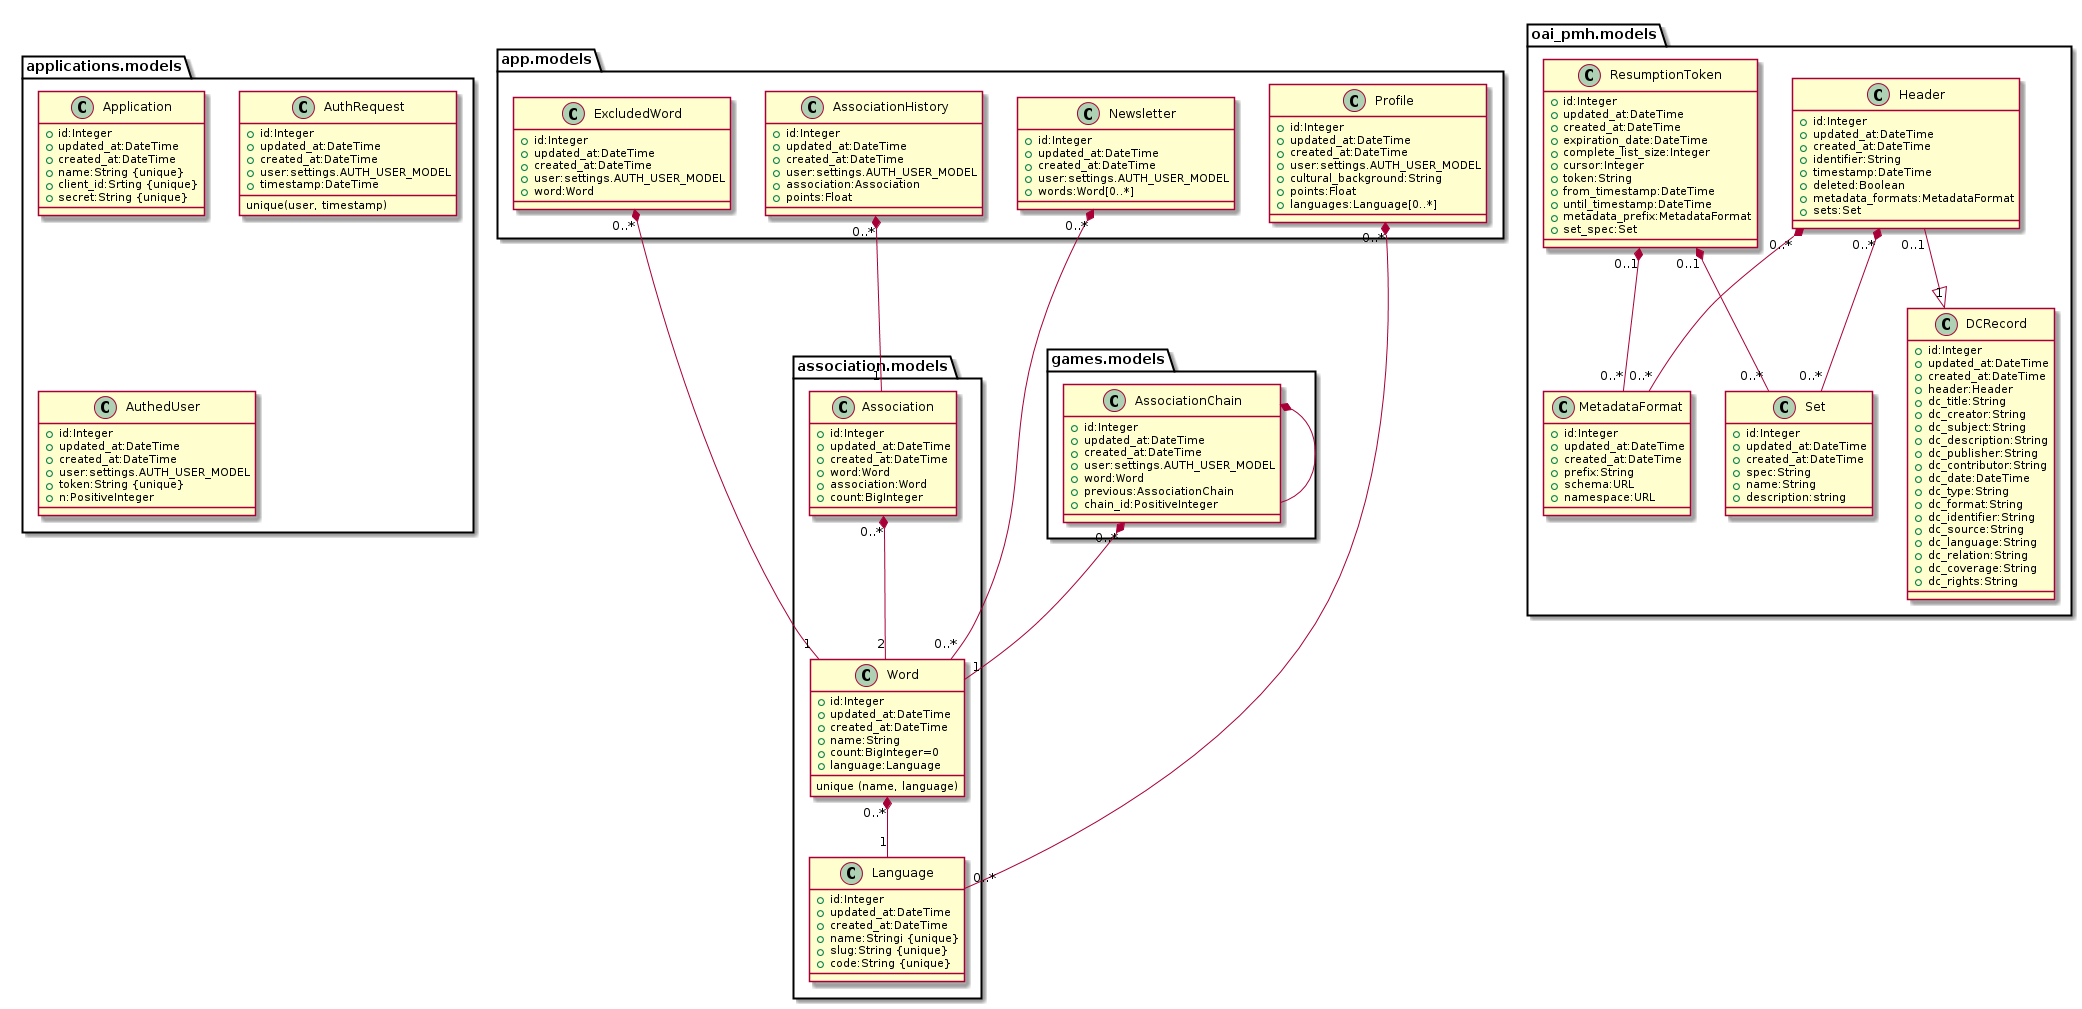
\includegraphics[width=\textwidth]{images/uml.png}
	\caption{UML des TIMA Datenmodells}
	\label{fig:uml}
\end{figure}

Das Modell \texttt{Language} repräsentiert die verfügbaren Sprachen der Wörter, das Modell \texttt{Word} die einzelnen Wörter, wobei ein Wort, wenn es in mehreren Sprachen existiert, für jede Sprache einen eigenen Eintrag hat und das Modell \texttt{Association} die Assoziation zwischen zwei Wörtern. Zusätzlich wird bei einem Wort gespeichert, wie oft dieses gefragt wurde und bei der Assoziation wie häufig diese gegeben wurde.

Die Modelle des Moduls \texttt{app.models} behandeln grundlegende Funktionen des Benutzermanagements. So zum Beispiel das Modell \texttt{Profile}, das den Kulturellen Hintergrund, die Punktzahl und die Sprachen für die ein Benutzer assoziiert hat, speichert. In dem Modell \texttt{AssociationHistory} wird die gesamte Assoziationsgeschichte eines Benutzers gespeichert, mit den jeweils für eine Assoziation erhaltenen Punkte. Das Modell \texttt{ExcludeWord} enthält für jeden Benutzer die Wörter, die er übersprungen hat (vgl. \hyperref[subsec:excludewords]{Abschnitt \ref*{subsec:excludewords}}), diese werden automatisch nach sieben Tagen gelöscht. Das letzte Modell in diesem Modul speichert für jeden Benutzer welche Worte er in seinem Newsletter empfangen möchte (vgl. \hyperref[subsec:newsletter]{Abschnitt \ref*{subsec:newsletter}}).

Das Modul \texttt{games.models} enthält Modelle die für die verschiedenen Spiele wichtig sind. Dies ist im Moment nur AssoziationsKette (vgl. \hyperref[subsec:games]{Abschnitt \ref*{subsec:games}}), hierfür werden in dem Modul \texttt{AssociationChain} die letzte/aktuelle Assoziationskette eines Benutzer gespeichert. Diese wird bei jedem Start eines Spieles gelöscht.

Für die Kommunikation zwischen App und Backend, insbesondere die schreib Zugriffe (vgl. \hyperref[sec:api]{Abschnitt \ref*{sec:api}}), zu autorisieren und dem speichert der nötigen Informationen dient das Modul \texttt{applications.models}. Das Modell \texttt{Application} speichert die Apps, die Autorisiert sind, mit den nötigen Daten für die Autorisierung (vgl. \hyperref[subsec:autorisierte_anfragen]{Abschnitt \ref*{subsec:autorisierte_anfragen}}). Die beiden anderen Modell in diesem Modul \texttt{AuthRequest} und \texttt{AuthedUser} speichern die nötigen Information für einen Benutzer der sich authentifizieren möchte und hat.

Das letzte Modul und die beinhalteten Modell sind für das OAI-PMH erforderlich siehe dafür (vgl. \hyperref[sec:oai-pmh]{Abschnitt \ref*{sec:oai-pmh}}).

\section{Webfrontend}
Das Webfrontend ist die Hauptanlaufstelle für Benutzer. Hierüber kann er sowohl anonym als auch angemeldet Assoziationen eingegeben, Wörter und
deren Assoziationen ansehen und weitere Funktionen (Rangliste, Statistik)
aufrufen.

Das Webfrontend basiert auf Django, wurde zusätzlich zu HTML mit Bootstrap und JQuery erstellt, sowie zur Visualisierung D3.

Im folgenden werden nun einige Funktionalitäten noch einmal einzeln kurz erläutert und beschrieben.

\subsection{Wortselektierungsalgorithmus}\label{subsec:wortselektierungsalgorithmus}
In diesem Abschnitt wird die Funktionsweise des Wortselektierungsalgorithmus genauer beschrieben. Der Wortselektierungsalgorithmus ist zuständig für das auswählen der Worte die assoziiert werden sollen. Folgende Anforderungen sollen dabei erfüllt werden:

\begin{itemize}
	\item Jedes Wort soll möglichst mindestens eine Assoziation haben.
	\item Jeder Benutzer soll möglichst zu jedem Wort mindestens eine Assoziation geben.
	\item Wörter, die wenig assoziiert wurden, entweder insgesamt oder von einem einzelnen Benutzer, bevorzugen.
	\item Wörter sollen ausgeschlossen werden können, um z.B. zu verhindern, dass das selbe Wort mehrmals hintereinander kommt.
\end{itemize}

Der Algorithmus der diese Anforderungen erfüllt sieht folgendermaßen aus:

\begin{lstlisting}[basicstyle=\ttfamily,
backgroundcolor=\color{lightgray},
showspaces=false,
showstringspaces=false,
showtabs=false,
columns=fixed,
frame=lines,
numbers=left,
numbersep=5pt,
breaklines=true,
captionpos=t,
caption=Wortselektierungsalgorithmus]
w = [alle Worter einer Sprache]
w = w - [alle auszuschließenden Wörter]
if ( Annonymer Benutzer )
    w = [15 Wörter mit niedrigstem Häufigkeit aus w]
else
    w = w - [alle auszuschließenden Wörter des Benutzers]
    w = [15 Wörter mit niedrigstem Auftreten in der AssociationHistory des Buntzers1 aus w]
return [zufälliges Wort aus w]
\end{lstlisting}

\subsection{ExcludeWords}\label{subsec:excludewords}
Falls ein Benutzer zu einem Wort keine Assoziation einfällt, hat er die Möglichkeit das Wort zu überspringen. Damit er nicht ständig danach gefragt wird (vgl. \hyperref[subsec:wortselektierungsalgorithmus]{Abschnitt \ref*{subsec:wortselektierungsalgorithmus}}), wird das Wort auf eine Ausschlussliste gesetzt. Einträge die älter als 7 Tage sind werden automatisch von der Liste gelöscht. Zu diesem Zeitpunkt, wird der Benutzer dann wieder gefragt dieses Wort zu assoziieren.

\subsection{Spiele}\label{subsec:games}
Die Idee mit den Spielen kam hauptsächlich durch die Apps (vgl. \hyperref[sec:spiele]{Abschnitt \ref*{sec:spiele}}). Allerdings haben wir uns dazu entschieden einzelne Spiele auch auf der Website anzubieten. Derzeit ist nur das Spiel AssoziationsKette verfügbar.

\subsection{Newsletter}\label{subsec:newsletter}
Ein weiteres Feature über das TIMA verfügt ist der Newsletter. Hier kann jeder Benutzer Wörter auswählen, die ihn interessieren und wöchentlich darüber einen Newsletter erhalten, in dem zu jedem Wort die Assoziationen mit deren Häufigkeit enthalten sind.

\section{API}\label{sec:api}
Damit die verschiedenen Apps mit der TIMA Datenbank kommunizieren können, haben
wir uns entschieden eine umfangreiche API zu implementieren. Diese lässt sich
grob in drei Teile gliedern. Zum einen gibt es die Anfragen, die keiner
Autorisierung bedürfen, zweitens jene die einer Autorisierung erfordern und
drittens eine OAI-PMH Schnittstelle.

Eine komplette Dokumentation der API ist in der Datei API.md\footnote{\url{https://github.com/Tima-Is-My-Association/TIMA/blob/master/API.md}} im git zu finden.

Im folgenden Abschnitt werden die einzelnen API Anfragen die keiner Autorisierung bedürfen näher erläutern, im darauffolgenden Abschnitt die, welche eine Autorisierung benötigen. Dort wird ebenfalls der Autorisierungsprozess näher erläutert. Zum Schluss wird dann noch ein Abschnitt zu OAI-PMH folgen.

\subsection{Nicht autorisierte Anfragen}
Die API-Anfragen, die keiner Autorisierung bedürfen sind allgemeine Anfragen, an die Assoziationsdatenbank, die auch über die Webseite ohne eine Anmeldung erfolgen können.

\paragraph{Rangliste} Eine dieser Anfragen ist die nach der Rangliste. Es werden keine weiteren Angaben benötigt und als Antwort kommt ein JSON-Object, das eine Liste der Benutzer enthält, mit den gleichen Daten wie sie über die Webseite einsehbar sind.

\paragraph{Statistik} Ebenso ist die Statistik über die API abfragbar.

\paragraph{Sprachen} Es kann eine Liste aller Sprachen in TIMA angefordert werden, hier ist neben dem Namen, der Sprach-Code in der Antwort enthalten, der bei vielen anderen Anfragen als Parameter angegeben werden muss.

\paragraph{Wörter} Um entweder ein einzelnes Wort oder eine Liste von Wörtern ist diese Anfrage bestimmt. Es können optional Wort-IDs, Sprache oder ein Limit für die Anzahl der Assoziationen pro Wort angegeben werden. Das JSON-Objekt der Antwort enthält unter anderem zu jedem Wort einen Link zur Website des Wortes, ein Link zu dieser Anfrage mit der Auswahl auf das einzelne Wort und der OAI-PMH identifier des Wortes.

\subsection{Autorisierte Anfragen}\label{subsec:autorisierte_anfragen}
Zum einem soll man sich über die Apps auf die Anmelden können, zum anderen soll nicht jede beliebige App schreib zugriff auf die TIMA Datenbank haben. Aus diesem Grund war es erforderlich, dass einige API Anfragen einer Autorisierung bedürfen.

Um dies zu realisieren haben wir uns zunächst bestehende Frameworks wie zum Beispiel OAuth2 angeschaut und getestet in wie weit diese unseren Anforderungen genügen. Dies hat allerdings zu keinen zufriedenstellendem Ergebnis geführt, weswegen wir entschieden haben dies selbstständig zu implementieren.

Die grundlegenden Anforderungen die wir dabei hatten sind wie folgt:
\begin{enumerate}
	\item sichere Authentisierung einer App
	\item sichere Authentisierung eines Benutzers
	\item sicherstellen das spätere Anfragen von einem Authentisierten Benutzer kommen
\end{enumerate}

\begin{figure}[!h]
	\centering
	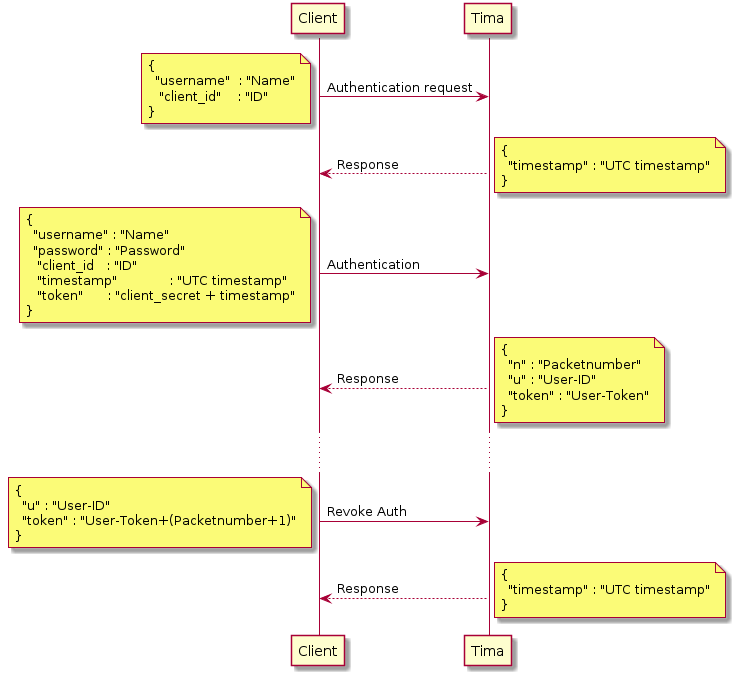
\includegraphics[width=\textwidth]{images/auth.png}
	\caption{Authentisierungsprozess}
	\label{fig:auth}
\end{figure}

In \hyperref[fig:auth]{Abbildung \ref*{fig:auth}} ist der Authentisierungsprozess schematisch Dargestellt. Der Client ist dabei eine App, über die sich ein Nutzer authentisieren möchte. Die App verfügt zum einen über eine \texttt{client\_id} und über ein \texttt{secret}, beides von TIMA vergebene eindeutige zufällige Strings. Der Authentisierungsprozess läuft wie folgt ab.
\begin{enumerate}
	\item Eine App sendet eine Anfrage an TIMA mit dem \texttt{username} des Benutzers und der \texttt{client\_id}. TIMA prüft diese beiden Werte auf Existenz und antwortet entweder mit \textbf{200} (HTTP Response Code) und dem aktuellen Zeitstempel oder mit \textbf{404}.
	\item Als nächstes sendet die App die eigentliche Authentisierungsanfrage. Mit \texttt{username} und \texttt{password} des Benutzers, \texttt{client\_id} der App, dem Zeitstempel der Antwort der letzten Anfrage und einem \texttt{token} das aus dem \texttt{secret} der App und dem Zeitstempel geniert wird (SHA512).
	\item TIMA antwortet wenn die Authentisierung erfolgreich war mit \textbf{200} und den folgenden drei Werten:
	\begin{itemize}
		\item[n] Paketnummer jeden Anfrage einer App muss diese um eins nach oben zählen. Als Wertebereich ist uint32 zubenutzen.
		\item[u] eine eindeutige Benutzer-ID, die bei jeder Anfrage mit zusenden ist
		\item[token] einem zufälligen String der bei jeder Anfrage zusammen mit \texttt{n}, der Paketnummer, in einem SHA512 Hash zu senden ist
	\end{itemize}
\end{enumerate}

\subsection{OAI-PMH}\label{sec:oai-pmh}
Bei OAI-PMH (Open Archives Initiative - Protocol for Metadata Harvesting)
handelt es sich um ein auf XML basierendes Protokoll zum sammeln von Metadaten.
Diese haben wir implementiert und wir liefern darüber Metadaten zu den
einzelnen Wörtern aus und in einem sehr geringem Maße über die Benutzer.
%TODO mehr!!
\chapter{Apps und Webseite}
Die Apps und die Webseite sollen die Verwendung vom TIMA für möglichst
viele Endnutzer möglich machen.

\section{Webseite}
Die Webseite bzw. das Webfrontend ist die Hauptanlaufstelle für Nutzer. Hierüber kann er sowohl anonym als auch angemeldet Assoziationen eingegeben, Wörter und
deren Assoziationen ansehen und weitere Funktionen wie die Rangliste und andere Statistiken aufrufen.

Das Webfrontend basiert auf Django, wurde zusätzlich zu HTML mit Bootstrap und JQuery erstellt. Zur Visualisierung von Assoziationsgraphen wurde D3.js verwendet.

\section{Apps}
De Apps sollen die Verwendung von TIMA ohne Webbrowser ermöglichen. Durch Apps wird besonders für mobile Geräte die Nutzung vereinfacht.
In einer erste Variante der App wurden grundlegende Funktionen der
Webseite nachgebaut. Dies diente unter anderem der Entwicklung der API, um etwaige
Fehler im Protokoll oder Verbesserungen dessen aufzuzeigen und zu beheben.

\subsection{Bibliothek}
Als Bibliothek wurde sich für Qt5 entschieden Aufgrund der weitreichenden
Unterstützung der Bibliothek auf verschiedenen Endgeräten. Hier ist besonders darauf hinzuweisen, das Qt5 sowohl auf Andriod als auch auf iOS läuft und so nicht die gleiche App für beide Betriebssysteme geschrieben werden muss.

\subsection{Aufbau}
Die innere Logik wird durch einen Zustandsautomaten dargestellt um
Mehrfachanfragen zu vermeiden und eine einfache Fehlerkorrektur zu ermöglichen.
In \hyperref[fig:uml_automata]{Abbildung \ref*{fig:uml_automata}} wird der Zusammenhang der einzelnen
Zustände angezeigt. Das wechseln der Zustände wird ausschließlich über die
Signale geregelt, die mit Qt implementiert sind.
\begin{figure}[!h]
	\centering
	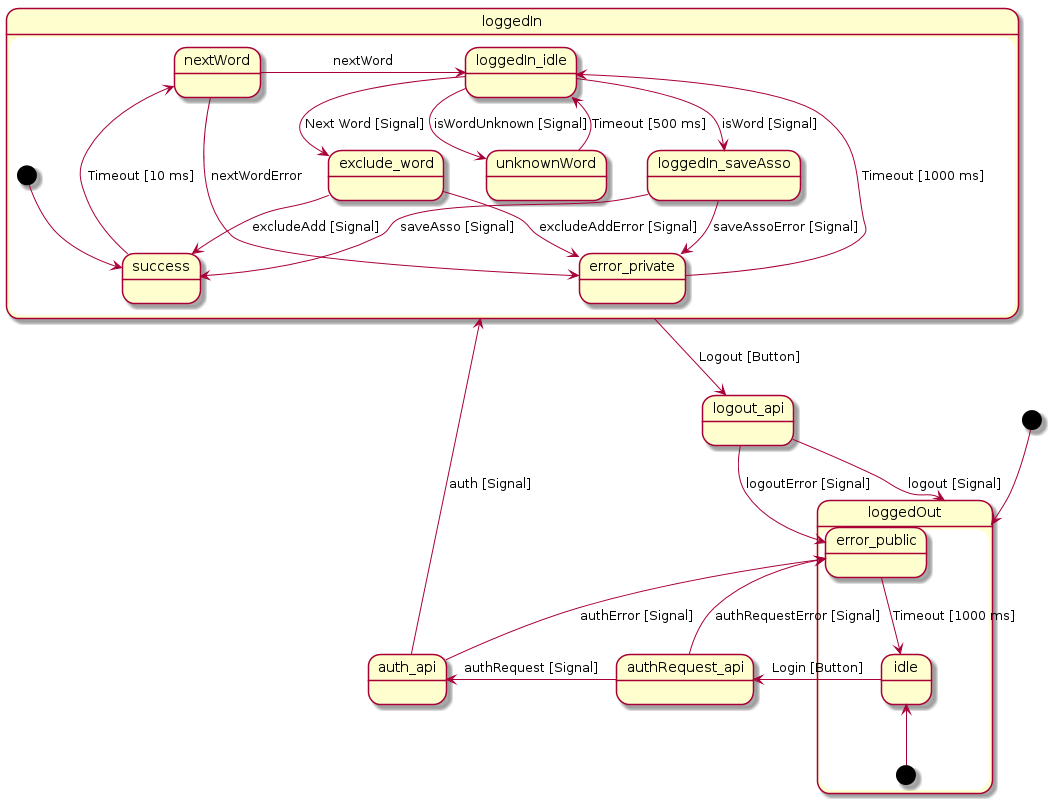
\includegraphics[width=\textwidth]{../UML/app_automata.png}
	\caption{UML State Diagramm des Appzustandsautomaten}
	\label{fig:uml_automata}
\end{figure}

\section{Sicherheit}
Die Sicherheit hat bei der Entwicklung eine große Rolle gespielt. Jede App nutzt die in \hyperref[subsec:authentifizierte_anfragen]{Abschnitt \ref*{subsec:authentifizierte_anfragen}} vorgestellte Autorisierungsmethode um  mit der API zu kommunizieren.  Dies dient dazu, dass lediglich von TIMA
akzeptierte Apps, Schreibrechte auf der Datenbank haben. Das Auslesen
der Informationen bleibt davon jedoch unangetastet, sofern es sich nicht um benutzerspezifische Daten handelt, und ist nach wie vor für
jeden offen.

\chapter{ausblick}

\chapter{Zusammenfassung}

\printbibliography
\end{document}
